\documentclass[11pt,a4paper]{article}

\usepackage[margin=2.2cm]{geometry}
\usepackage{amsmath,amssymb}
\usepackage{graphicx}
\usepackage{booktabs}
\usepackage{float}
\usepackage{xcolor}
\usepackage{enumitem}
\usepackage{microtype}
\usepackage[hidelinks]{hyperref}
\sloppy

\definecolor{accent}{HTML}{1D4ED8}
\definecolor{muted}{HTML}{4B5563}

\title{\textbf{GWLab: Deterministic Gravitational-Wave Matched Filtering and Bayesian Parameter-Estimation Laboratory}\\[0.4em]
\large Technical Report, Mathematical Specification, and Validation Record}
\author{GWLab Project Release Candidate (Phase 6C)}
\date{November 26, 2026}

\begin{document}
\maketitle

\begin{abstract}
\textbf{GWLab} is a reproducible scientific computing and web visualization laboratory for compact binary coalescence (CBC) gravitational-wave signal analysis, frequency-domain matched filtering, and Bayesian nested-sampling parameter-estimation forensics. The system pairs a frozen Python scientific engine (\texttt{gw\_inference}) with a FastAPI service (\texttt{src/gwlab/api/}) and a Next.js~\texttt{16.4.6} frontend (\texttt{frontend/}). All interactive signal, noise, and matched-filter evaluations execute deterministically on synthetic data, while Bayesian posterior and multi-seed evidence views read directly from frozen, provenance-tracked nested-sampling archives. Under the synthetic benchmark configuration ($4\,\mathrm{s}$ segment at $2048\,\mathrm{Hz}$, active band $[20, 512]\,\mathrm{Hz}$, Model~2 Whittle Gaussian likelihood), the Stage~6C Run~A anchor achieves $\ln Z = 201646.1413 \pm 0.2374\,\mathrm{nats}$ ($11{,}951$ weighted samples, $\eta$ upper-1\% prior-range mass $= 38.57\%$), and the Stage~5G.2 two-seed diagnostic records $|\Delta \ln Z| = 2.9720\,\mathrm{nats}$ (ratio $8.92$). The repository passes $517/517$ backend tests, $86\%$ statement coverage on \texttt{src/gwlab/}, and $21/21$ Playwright route-viewport checks.
\end{abstract}

\tableofcontents
\newpage

\section{Introduction and Project Objectives}
Gravitational-wave parameter estimation for compact binary coalescences relies on accurate frequency-domain waveform phasing, calibrated noise power spectral density (PSD) estimation, inner-product matched filtering, and likelihood-normalized Bayesian evidence integration~\cite{Finn1992,CutlerFlanagan1994}. GWLab was engineered to separate a strictly deterministic, unit-tested numerical core (\texttt{gw\_inference}) from a read-only interactive laboratory (\texttt{gwlab}) so that researchers can inspect waveform dynamics, colored-noise Welch estimation, matched-filter signal-to-noise ratio (SNR) time series, and saved nested-sampling posteriors without launching stochastic samplers from the presentation layer.

The core objectives are:
\begin{enumerate}[leftmargin=1.5em]
    \item \textbf{Convention consistency:} Enforce unified Fourier, Parseval, and inner-product conventions across waveform generation, PSD estimation, matched filtering, and Whittle likelihood evaluation.
    \item \textbf{Deterministic interactivity:} Expose TaylorF2 $3.5\mathrm{PN}$ waveforms, synthetic colored Gaussian noise + Welch PSD estimation, and matched filtering via typed FastAPI endpoints.
    \item \textbf{Read-only archive provenance:} Serve saved Stage~6C Run~A posterior samples and Stage~5G.2 two-seed evidence comparisons with explicit scientific qualifications and zero live sampler execution.
    \item \textbf{Reproducible verification:} Maintain automated regression coverage across backend physics, API schemas, frontend TypeScript/ESLint/build checks, and multi-viewport Playwright UI tests.
\end{enumerate}

\section{TaylorF2 3.5PN Waveform Model}
For a non-spinning binary with component masses $m_1 \ge m_2$, total mass $M = m_1 + m_2$, symmetric mass ratio $\eta = m_1 m_2 / M^2 \in (0, 0.25]$, and chirp mass $\mathcal{M}_c = M \eta^{3/5}$, GWLab implements the stationary-phase frequency-domain \texttt{TaylorF2} approximant~\cite{SathyaprakashDhurandhar1991,Buonanno2009} with Newtonian amplitude and $3.5\mathrm{PN}$ phase:
\begin{equation}
\tilde{h}(f) = \mathcal{A}(f)\,e^{-i\Psi(f)}, \qquad f \in [f_{\min}, f_{\mathrm{term}}],
\end{equation}
where the upper cutoff $f_{\mathrm{term}} = \min(f_{\mathrm{end}}, f_{\mathrm{ISCO}})$ is bounded by the Schwarzschild innermost stable circular orbit frequency,
\begin{equation}
f_{\mathrm{ISCO}} = \frac{c^3}{6^{3/2}\,\pi G M}.
\end{equation}
The restricted Newtonian inspiral amplitude scaling with luminosity distance $d_L$ is
\begin{equation}
\mathcal{A}(f) = \sqrt{\frac{5}{24}}\,\frac{G^{5/6}\mathcal{M}_c^{5/6}\,c^{-3/2}}{\pi^{2/3}\,d_L}\,f^{-7/6},
\end{equation}
and the $3.5\mathrm{PN}$ Fourier phase expansion in the post-Newtonian velocity parameter $v = (\pi G M f / c^3)^{1/3}$ is
\begin{equation}
\Psi(f) = 2\pi f t_c - \phi_c - \frac{\pi}{4} + \frac{3}{128\eta v^5}\sum_{k=0}^{7} \alpha_k(\eta)\,v^k,
\end{equation}
where $t_c$ and $\phi_c$ denote the coalescence arrival time and phase, respectively. For the Stage~6C reference injection, $\mathcal{M}_c = 28.0956\,M_\odot$, $\eta = 0.2471$, $d_L = 410.0\,\mathrm{Mpc}$, $t_c = 2.0\,\mathrm{s}$ (in the $4\,\mathrm{s}$ filter/inference frame), and $\phi_c = 0.0\,\mathrm{rad}$.

\section{Noise Modeling, Analytical PSD Proxy, and Welch Estimation}
\subsection{Analytical PSD Proxy Qualification}
GWLab models detector noise via a one-sided power spectral density $S_n(f)$ and amplitude spectral density $\mathrm{ASD}(f) = \sqrt{S_n(f)}$. Crucially, the default \texttt{aligo\_representative} model is a \textbf{custom, regularized analytical aLIGO-like PSD proxy} designed for controlled numerical benchmarking; it is \textbf{not} an official LIGO design-sensitivity curve or measured LIGO Hanford (H1) strain spectrum. A flat white-noise reference (\texttt{flat}) is also supported.

\subsection{Synthetic Colored Noise and Welch PSD}
Given $N$ time-domain samples at $\Delta t = 1/f_s$ ($\Delta f = 1/T$), synthetic stationary colored Gaussian noise is generated by drawing zero-mean complex Gaussian Fourier modes with variance scaled to $\frac{1}{2} S_n(f_k)/\Delta f$ and transforming via inverse real FFT. Off-source PSD estimation uses Welch's overlapped segmented periodogram~\cite{Welch1967} with a Tukey cosine-tapered window ($\alpha = 0.25$, $T_{\mathrm{seg}} = 4.0\,\mathrm{s}$, $50\%$ overlap). For a $64.0\,\mathrm{s}$ synthetic observation ($K = 31$ segments), the overlap-variance inflation factor is $\kappa_{\mathrm{overlap}} = 1.3823$, yielding an effective degrees-of-freedom count $\nu_{\mathrm{eff}} = 44.85$. Figure~\ref{fig:psd_asd} compares the analytical proxy against the deterministic Welch estimate (\texttt{seed=7101}).

\begin{figure}[H]
    \centering
    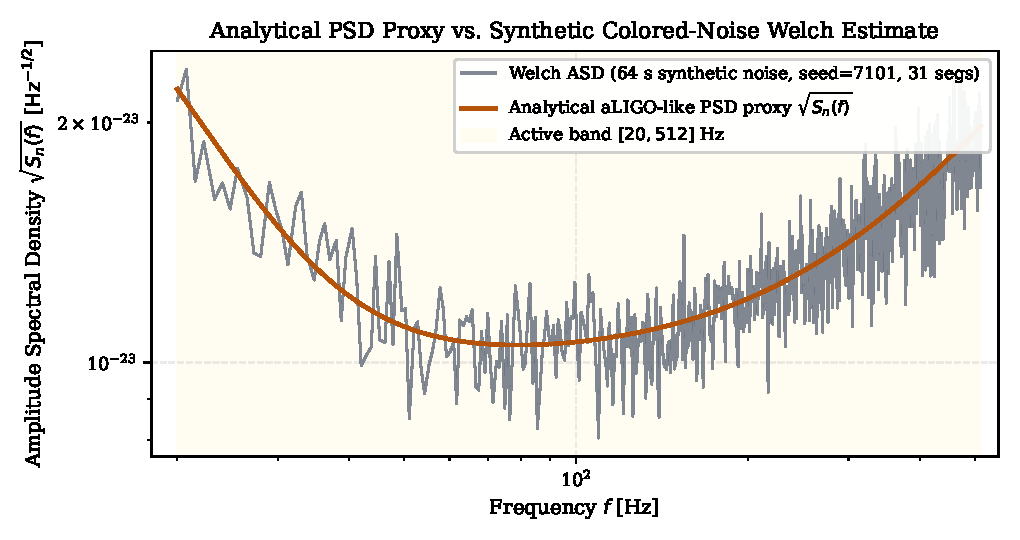
\includegraphics[width=0.92\textwidth]{figures/fig1_psd_asd.pdf}
    \caption{Comparison of the custom analytical aLIGO-like ASD proxy $\sqrt{S_n(f)}$ (solid amber) and the Tukey-windowed Welch ASD estimate (gray) computed from a $64\,\mathrm{s}$ synthetic colored Gaussian noise realization (\texttt{seed=7101}, $31$ segments, $\alpha=0.25$, $50\%$ overlap) over the active band $[20, 512]\,\mathrm{Hz}$.}
    \label{fig:psd_asd}
\end{figure}

\section{Matched Filtering and Optimal SNR}
Using the discrete one-sided noise-weighted inner product over the active positive-frequency index set $\mathcal{K}_+$ ($f_k \in [20, 512]\,\mathrm{Hz}$, $\Delta f = 0.25\,\mathrm{Hz}$),
\begin{equation}
\langle a \mid b \rangle = 4\,\Delta f\,\operatorname{Re}\sum_{k \in \mathcal{K}_+} \frac{\tilde{a}^*(f_k)\,\tilde{b}(f_k)}{S_n(f_k)},
\end{equation}
the template normalization is $\sigma_h = \sqrt{\langle h \mid h \rangle}$, which equals the expected optimal matched-filter SNR $\rho_{\mathrm{opt}}$ for a zero-mismatch signal. The complex matched-filter SNR time series against data $\tilde{d}(f) = \tilde{h}_{\mathrm{inj}}(f) + \tilde{n}(f)$ is evaluated via inverse FFT~\cite{Allen2012}:
\begin{equation}
\rho(t_j) = \frac{4\,\Delta f}{\sigma_h} \sum_{k \in \mathcal{K}_+} \frac{\tilde{d}(f_k)\,\tilde{h}_{\mathrm{tmpl}}^*(f_k)}{S_n(f_k)}\,e^{+i 2\pi f_k t_j}.
\end{equation}
Taking $|\rho(t_j)|$ analytically maximizes over the unknown coalescence phase $\phi_c$. Under the Realization~01 benchmark (\texttt{seed=7151}), the optimal template SNR is $\rho_{\mathrm{opt}} = 45.3153$. As shown in Figure~\ref{fig:matched_filter}, a zero-mismatch template recovers a peak SNR of $44.28$ near $t_c = 2.0\,\mathrm{s}$, whereas a $+2.5\,M_\odot$ chirp-mass mismatch degrades the peak SNR to $34.43$.

\begin{figure}[H]
    \centering
    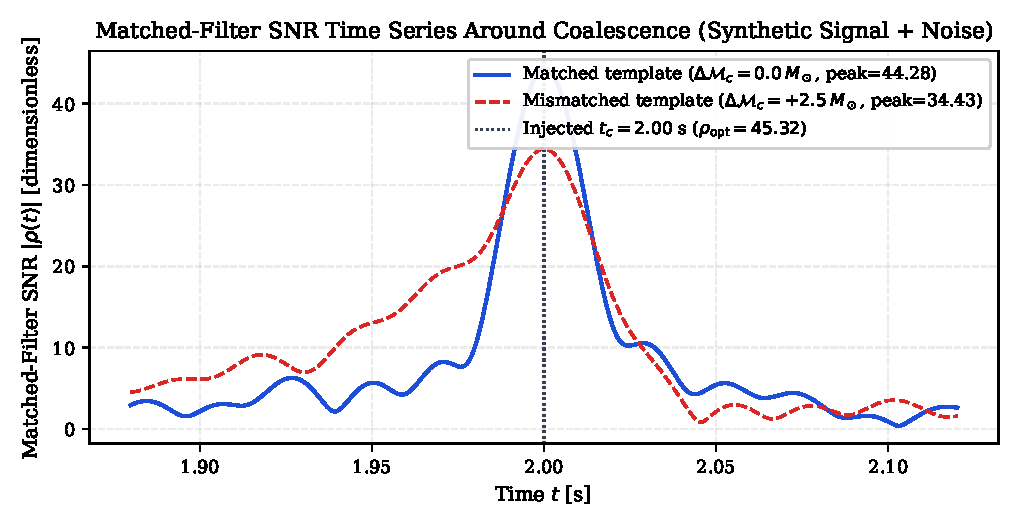
\includegraphics[width=0.92\textwidth]{figures/fig2_matched_filter_snr.pdf}
    \caption{Matched-filter SNR magnitude $|\rho(t)|$ around coalescence for synthetic injection + colored Gaussian noise (\texttt{seed=7151}, $\rho_{\mathrm{opt}} = 45.3153$). A matched template ($\Delta\mathcal{M}_c = 0.0\,M_\odot$) recovers a peak of $44.28$, while a $\Delta\mathcal{M}_c = +2.5\,M_\odot$ mismatch drops the peak to $34.43$.}
    \label{fig:matched_filter}
\end{figure}

\section{Model 2 Whittle Likelihood and Active Band}
Bayesian parameter estimation in the frozen benchmark campaign uses the frequency-domain Whittle Gaussian log-likelihood (Model~2) over $\mathcal{K}_+$ ($[20, 512]\,\mathrm{Hz}$):
\begin{equation}
\ln \mathcal{L}(\theta) = -\frac{1}{2}\sum_{k \in \mathcal{K}_+} \left[ \frac{4\,\Delta f\,\big|\tilde{d}(f_k) - \tilde{h}(f_k;\theta)\big|^2}{S_n(f_k)} + \ln\!\left(\frac{\pi S_n(f_k)}{2\,\Delta f}\right) \right],
\end{equation}
preserving the exact normalization constant required for Bayesian evidence $\ln Z$. Model~3 (Student-$t$ heavy-tailed likelihood) remains frozen/specified in design documents and is \textbf{not} approved as production inference.

\section{Bayesian Posterior Results and Evidence Provenance}
\subsection{Stage 6C Run A Anchor Posterior}
The \texttt{/inference} explorer visualizes saved weighted nested-sampling~\cite{Skilling2006,Speagle2020} samples from \path{experiments/wp6_stage6c_anchor/run_a_anchor_samples.npz} (single-seed Run~A, \texttt{seed=8101}, $4\mathrm{D}$ parameter vector $\theta = (\mathcal{M}_c, \eta, t_c, \phi_c)$). Key archived metrics are summarized in Table~\ref{tab:stage6c} and Figure~\ref{fig:posteriors}. Notably, $38.57\%$ of posterior probability mass lies in the upper $1\%$ of the $\eta$ prior range ($\eta \ge 0.2485$), reflecting the equal-mass boundary geometry near the injected $\eta = 0.2471$.

\begin{table}[H]
    \centering
    \caption{Stage 6C Run A Anchor Summary (\texttt{run\_a\_anchor\_result.json}, single-seed \texttt{8101}).}
    \label{tab:stage6c}
    \begin{tabular}{ll}
        \toprule
        \textbf{Metric} & \textbf{Archived Value} \\
        \midrule
        Log-Evidence $\ln Z$ & $201646.1413 \pm 0.2374\,\mathrm{nats}$ \\
        Likelihood Evaluations & $500{,}657$ (raw) \\
        Weighted Posterior Samples & $11{,}951$ (Kish $N_{\mathrm{eff}} = 2867.4$) \\
        Wall / CPU Time & $514.83\,\mathrm{s}$ / $473.16\,\mathrm{s}$ \\
        Posterior mass in upper 1\% of $\eta$ prior & $38.57\%$ ($\eta \ge 0.2485$) \\
        \bottomrule
    \end{tabular}
\end{table}

\begin{figure}[H]
    \centering
    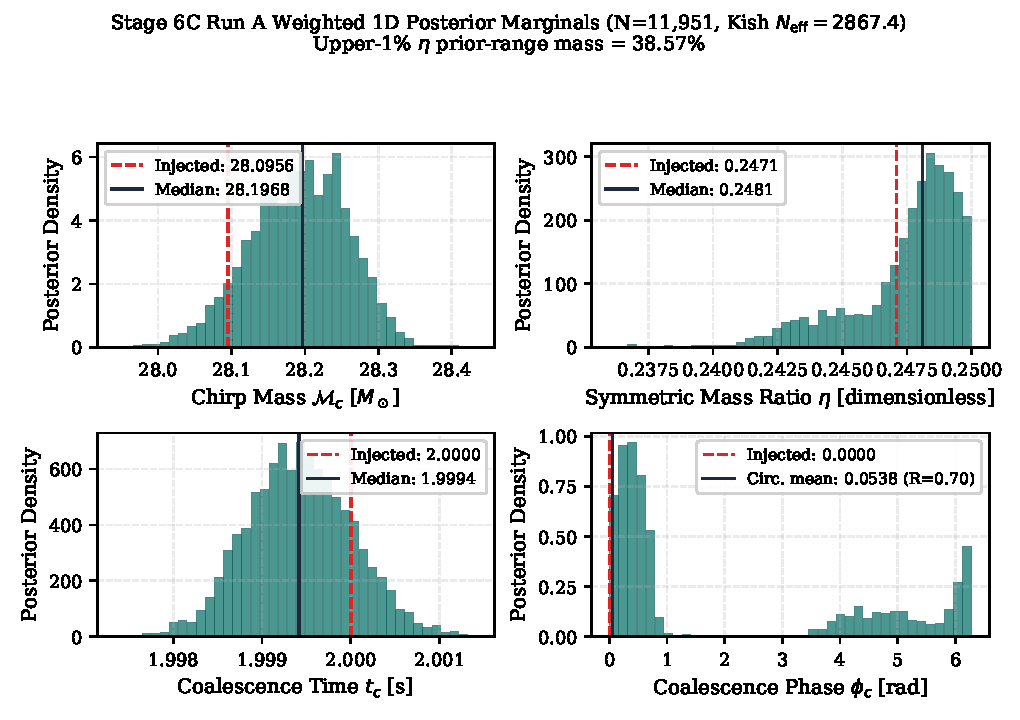
\includegraphics[width=0.95\textwidth]{figures/fig3_posterior_marginals.pdf}
    \caption{Weighted 1D marginal posterior densities for $\mathcal{M}_c$, $\eta$, $t_c$, and $\phi_c$ from the saved Stage~6C Run~A archive ($N = 11{,}951$ samples, Kish $N_{\mathrm{eff}} = 2867.4$). Dashed red lines indicate injected values; solid dark lines indicate posterior medians.}
    \label{fig:posteriors}
\end{figure}

\subsection{Stage 5G.2 Two-Seed Evidence Sensitivity}
The \texttt{/experiments} view compares the archived Stage~5G.2 two-seed pair (\texttt{base\_01\_plug\_inst\_s1}, \texttt{seed=8101}, $\ln Z = 201646.1413 \pm 0.2374\,\mathrm{nats}$ vs.\ \texttt{base\_01\_plug\_inst\_s2}, \texttt{seed=8201}, $\ln Z = 201643.1693 \pm 0.2338\,\mathrm{nats}$), shown in Figure~\ref{fig:two_seed}. The observed difference is $|\Delta \ln Z| = 2.9720\,\mathrm{nats}$ with quadrature-combined internal uncertainty $\sigma_\Delta = 0.3332\,\mathrm{nats}$, yielding a discrepancy ratio of $8.92$. \textbf{Qualification:} this ratio reflects internal sampler reporting under 1 degree of freedom; it is a sensitivity diagnostic, \emph{not} a calibrated frequentist significance, convergence proof, or coverage validation. Furthermore, \texttt{Stage 6C Run B} and \texttt{Seed 8301} remain unexecuted/proposed.

\begin{figure}[H]
    \centering
    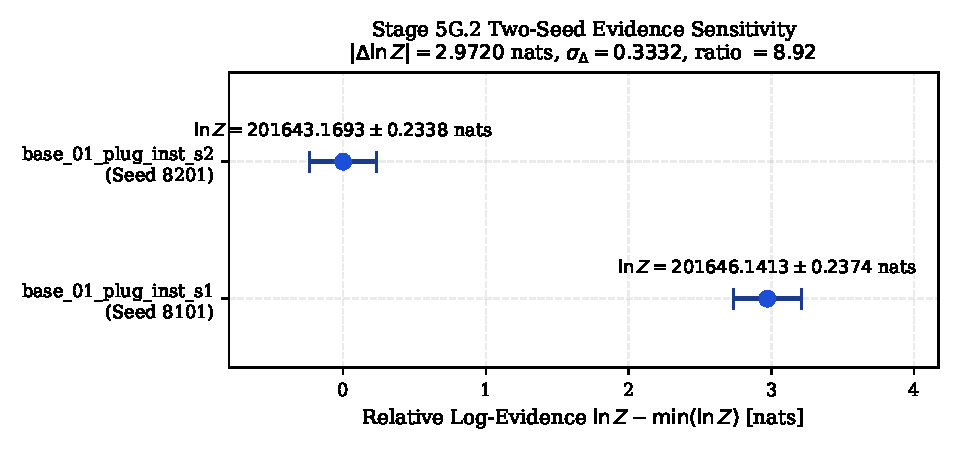
\includegraphics[width=0.88\textwidth]{figures/fig4_two_seed_evidence.pdf}
    \caption{Stage~5G.2 two-seed evidence comparison (\texttt{base\_01\_plug\_inst\_s1} vs.\ \texttt{base\_01\_plug\_inst\_s2}). The $2.9720\,\mathrm{nat}$ difference (ratio $8.92$) is a two-seed sensitivity diagnostic, not a convergence or coverage proof.}
    \label{fig:two_seed}
\end{figure}

\section{Software Architecture, API, and Reproducibility}
GWLab separates presentation from scientific computation:
\begin{itemize}[leftmargin=1.5em]
    \item \textbf{Frontend (\texttt{frontend/}):} Next.js~\texttt{16.4.6} App Router (\texttt{output: "standalone"}), React~19, TypeScript, Tailwind CSS, and KaTeX across seven routes (\texttt{/}, \texttt{/waveforms}, \texttt{/noise-and-psd}, \texttt{/matched-filtering}, \texttt{/inference}, \texttt{/experiments}, \texttt{/methods}).
    \item \textbf{Backend (\path{src/gwlab/api/}):} FastAPI service exposing \path{/api/status}, \path{/api/benchmarks/overview}, \path{/api/waveforms/generate}, \path{/api/waveforms/chirp-time}, \path{/api/noise/analyze}, \path{/api/matched-filter/evaluate}, \path{/api/inference/posterior}, and \path{/api/experiments/explorer}.
    \item \textbf{Configuration \& Packaging:} Centralized settings (\path{src/gwlab/config.py}) support \texttt{GWLAB\_DATA\_ROOT} (path-traversal-guarded read-only artifact root), \texttt{GWLAB\_CORS\_ORIGINS}, \texttt{NEXT\_PUBLIC\_API\_URL}, a cross-platform launcher (\path{scripts/launch_gwlab.py}), and multi-container Docker/Compose definitions (\texttt{Dockerfile.backend}, \texttt{Dockerfile.frontend}, \texttt{docker-compose.yml}).
\end{itemize}

\begin{table}[H]
    \centering
    \caption{Verification and Release-Readiness Summary (Phase 6A--6C).}
    \label{tab:validation}
    \begin{tabular}{lll}
        \toprule
        \textbf{Check} & \textbf{Result} & \textbf{Notes} \\
        \midrule
        Full Repository \texttt{pytest} & $517/517$ passing & Includes WP0--WP6 and GWLab suites \\
        GWLab Backend \& Config Tests & $62/62$ passing & \texttt{tests/test\_gwlab\_*.py} \\
        \texttt{src/gwlab/} Statement Coverage & $86\%$ ($788/911$) & Exceeds $85\%$ target \\
        Playwright E2E Matrix & $21/21$ passing & $7$ routes $\times$ $3$ viewports; $0$ errors/overflows \\
        TypeScript / ESLint / Prod Build & $0$ errors & \texttt{standalone} build verified; $7$ lint warnings \\
        Docker Build / Compose Run & Not executed locally & Configured; \texttt{docker} CLI absent on host \\
        \bottomrule
    \end{tabular}
\end{table}

\section{Limitations and Conclusion}
GWLab is validated as a documented local release candidate. Key operational boundaries remain: (1) all interactive waveforms, noise, and matched-filter runs use synthetic data and the custom \texttt{aligo\_representative} PSD proxy; (2) Bayesian posterior and experiment views are read-only reflections of archived runs; (3) Docker Compose execution has not yet been verified on a Docker-enabled host; and (4) while production runtime self-hosts $50$ bundled \texttt{.woff2} font files, clean \texttt{next build} execution still fetches Google Fonts at build time. Within these documented boundaries, GWLab provides a rigorous, reproducible gravitational-wave analysis workbench.

\begin{thebibliography}{9}
\bibitem{SathyaprakashDhurandhar1991}
B.~S. Sathyaprakash and S.~V. Dhurandhar, ``Choice of filters for the detection of gravitational waves from coalescing binaries,'' \emph{Phys. Rev. D}, vol.~44, pp.~3819--3834, 1991.

\bibitem{Finn1992}
L.~S. Finn, ``Detection, measurement, and gravitational radiation,'' \emph{Phys. Rev. D}, vol.~46, pp.~5236--5249, 1992.

\bibitem{CutlerFlanagan1994}
C.~Cutler and E.~E. Flanagan, ``Gravitational waves from merging compact binaries: How accurately can one extract the binary's parameters from the inspiral waveform?,'' \emph{Phys. Rev. D}, vol.~49, pp.~2658--2697, 1994.

\bibitem{Buonanno2009}
A.~Buonanno, B.~R. Iyer, E.~Ochsner, Y.~Pan, and B.~S. Sathyaprakash, ``Comparison of post-Newtonian templates for compact binary inspiral signals in gravitational-wave detectors,'' \emph{Phys. Rev. D}, vol.~80, p.~084043, 2009.

\bibitem{Allen2012}
B.~Allen, W.~G. Anderson, P.~R. Brady, D.~A. Brown, and J.~D.~E. Creighton, ``FINDCHIRP: An algorithm for detection of gravitational waves from inspiraling compact binaries,'' \emph{Phys. Rev. D}, vol.~85, p.~122006, 2012.

\bibitem{Welch1967}
P.~D. Welch, ``The use of fast Fourier transform for the estimation of power spectra: A method based on time averaging over short, modified periodograms,'' \emph{IEEE Trans. Audio Electroacoust.}, vol.~15, no.~2, pp.~70--73, 1967.

\bibitem{Skilling2006}
J.~Skilling, ``Nested sampling for general Bayesian computation,'' \emph{Bayesian Analysis}, vol.~1, no.~4, pp.~833--859, 2006.

\bibitem{Speagle2020}
J.~S. Speagle, ``\texttt{dynesty}: a dynamic nested sampling package for estimating Bayesian posteriors and evidences,'' \emph{Mon. Not. R. Astron. Soc.}, vol.~493, no.~3, pp.~3132--3158, 2020.
\end{thebibliography}

\end{document}
